\begin{frame}{Example: Step 1}
	$M = (r, b, mt, r)$, $EQUAL(0, 3)$
	
	\begin{itemize}
		\item Optimal route found with PNE: $(r_1, b_1, mt_1, r_2)$
		\item Dummy SR: $(r_1, b_1, mt_1, r_1)$; Upper Bound $UB = length(dummySR)$
	\end{itemize}

	\begin{figure}[h]
		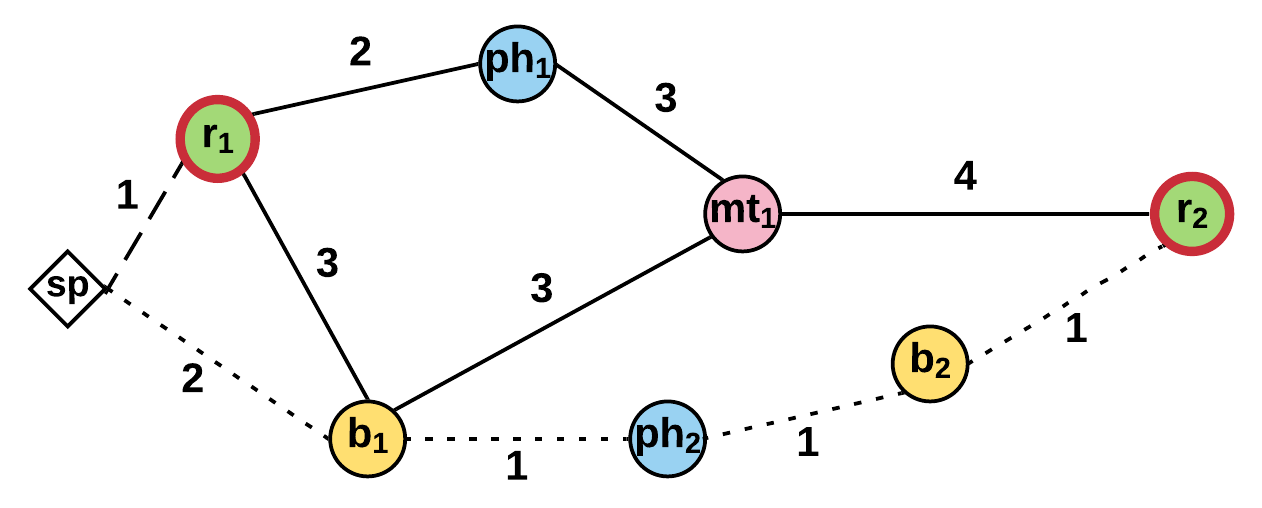
\includegraphics[scale=0.8]{Example_EO_1.png}
	\end{figure}
	
	\begin{table}[h]
		\centering
		\begin{tabular}{ |l|p{10cm}| } 
			\hline
			Step & Heap contents (PSR $R : length(R), heuristic(R)$) \\
			\hline
			\textcolor{red}{1} & \textcolor{red}{$(r_1 : 1, 5)$}, \textcolor{red}{$(r_2 : 5, 4)$} \\ 
			\hline
		\end{tabular}
	\end{table}
		
\end{frame}

\begin{frame}{Example: Step 2}
	$M = (r, b, mt, r)$, $EQUAL(0, 3)$

	\begin{figure}[h]
		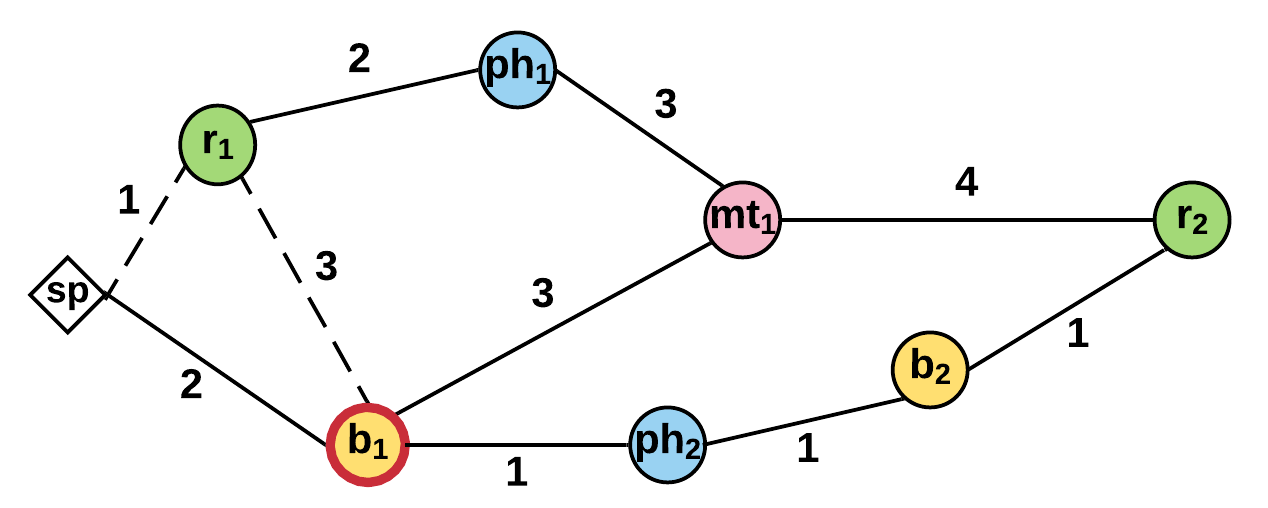
\includegraphics[scale=0.8]{Example_EO_2.png}
	\end{figure}
	
	\begin{table}[h]
		\centering
		\begin{tabular}{ |l|p{10cm}| } 
			\hline
			Step & Heap contents (PSR $R : length(R), heuristic(R)$) \\
			\hline
			1 & $(r_1 : 1, 5), (r_2 : 5, 4)$ \\ 
			\hline
			\textcolor{red}{2} & \textcolor{red}{$(r_1, b_1 : 4, 3)$}, $(r_2 : 5, 4)$ \\ 
			\hline
		\end{tabular}
	\end{table}

\end{frame}

\begin{frame}{Example: Step 8}
	$M = (r, b, mt, r)$, $EQUAL(0, 3)$
	
	\begin{figure}[h]
		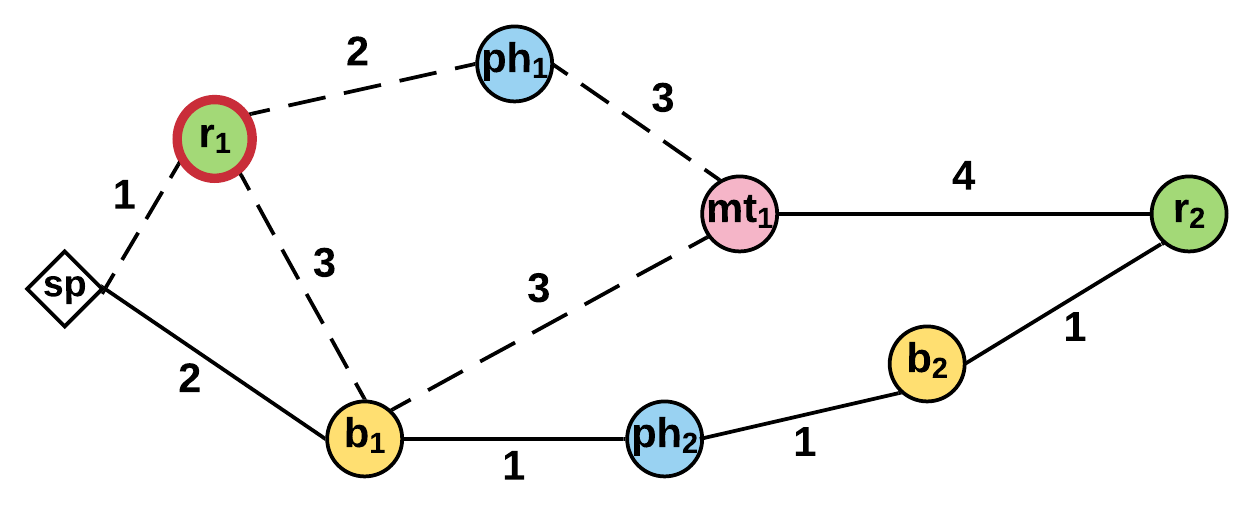
\includegraphics[scale=0.8]{Example_EO_8.png}
	\end{figure}
	
	Candidate SR: \textcolor{red}{$(r_1, b_1, mt_1, r_1 : 12, 0)$}
	
	\begin{table}[h]
		\centering
		\begin{tabular}{ |l|p{10cm}| } 
			\hline
			Step & Heap contents (PSR $R : length(R), heuristic(R)$) \\
			\hline
			7 & $(r_1, b_1, mt_1 : 7, 5), (r_2, b_1, mt_1 : 11, 4), (r_2, b_2, mt_1 : 11, 4),$ \newline $(r_1, b_2, mt_1 : 11, 5)$ \\ 
			\hline
			\textcolor{red}{8} & $(r_2, b_1, mt_1 : 11, 4), (r_2, b_2, mt_1 : 11, 4), (r_1, b_2, mt_1 : 11, 5)$ \\ 
			\hline
		\end{tabular}
	\end{table}

\end{frame}

\begin{frame}{Example: Step 9}
	$M = (r, b, mt, r)$, $EQUAL(0, 3)$
	
	\begin{figure}[h]
		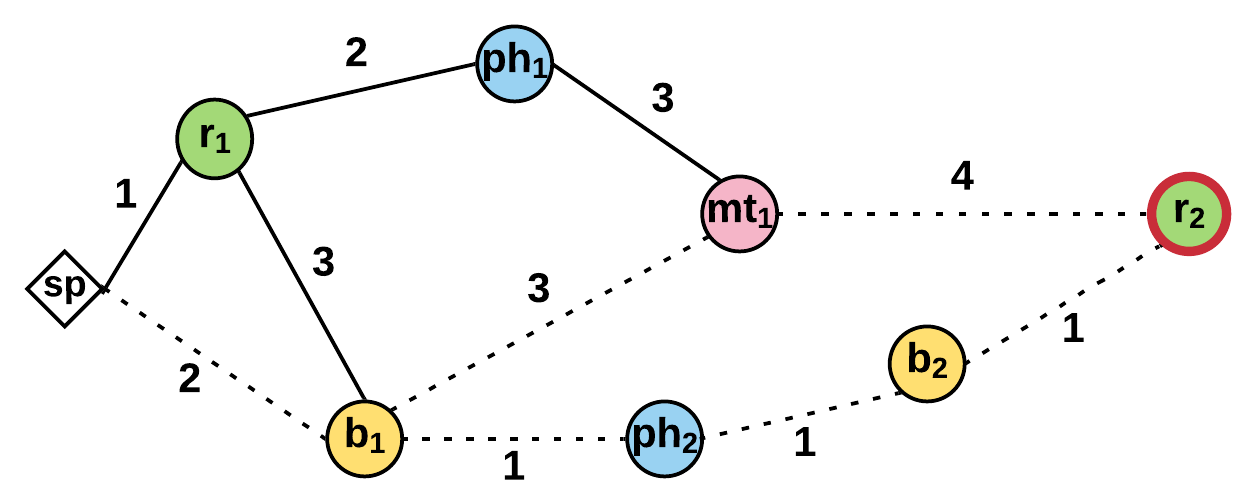
\includegraphics[scale=0.8]{Example_EO_9.png}
	\end{figure}
	
	Candidate SR: \textcolor{red}{$(r_2, b_1, mt_1, r_2 : 15, 0)$}

	\begin{table}[h]
		\centering
		\begin{tabular}{ |l|p{10cm}| } 
			\hline
			Step & Heap contents (PSR $R : length(R), heuristic(R)$) \\
			\hline
			8 & $(r_2, b_1, mt_1 : 11, 4), (r_2, b_2, mt_1 : 11, 4), (r_1, b_2, mt_1 : 11, 5)$ \\ 
			\hline
			\textcolor{red}{9} & $(r_2, b_2, mt_1 : 11, 4), (r_1, b_2, mt_1 : 11, 5)$ \\ 
			\hline
		\end{tabular}
	\end{table}

\end{frame}

%\begin{frame}{Example}
%
%	\begin{table}[]
%		\centering
%		\begin{tabular}{ |l|p{10cm}| } 
%			\hline
%			Step & Heap contents (PSR $R : length(R), heuristic(R)$) \\
%			\hline
%			1 & $(r_1 : 1, 5), (r_2 : 5, 4)$ \\ 
%			\hline
%			2 & $(r_1, b_1 : 4, 3), (r_2 : 5, 4)$ \\ 
%			\hline
%			3 & $(r_2 : 5, 4), (r_1, b_2 : 6, 5), (r_1, b_1, mt_1 : 7, 5)$ \\ 
%			\hline
%			4 & $(r_1, b_2 : 6, 5), (r_2, b_2 : 6, 5), (r_1, b_1, mt_1 : 7, 5) $ \\ 
%			\hline
%			5 & $(r_2, b_2 : 6, 5), (r_1, b_1, mt_1 : 7, 5)$,  \newline $(r_1, b_2, mt_1 : 11, 5)$ \\ 
%			\hline
%			6 & $(r_2, b_1 : 8, 3), (r_1, b_1, mt_1 : 7, 5) , (r_2, b_2, mt_1 : 11, 4), (r_1, b_2, mt_1 : 11, 5)$ \\ 
%			\hline
%			7 & $(r_1, b_1, mt_1 : 7, 5) , (r_2, b_1, mt_1 : 11, 4), (r_2, b_2, mt_1 : 11, 4), (r_1, b_2, mt_1 : 11, 5)$ \\ 
%			\hline
%			8 & $(r_2, b_1, mt_1 : 11, 4), (r_2, b_2, mt_1 : 11, 4), (r_1, b_2, mt_1 : 11, 5)$ \\ 
%			\hline
%			9 & $(r_2, b_2, mt_1 : 11, 4), (r_1, b_2, mt_1 : 11, 5)$ \\ 
%			\hline
%			10 & $ (r_1, b_2, mt_1 : 11, 5)$ \\ 
%			\hline
%			11 & $heap$ is empty \\ 
%			\hline
%		\end{tabular}
%	\end{table}
%
%\end{frame}